% Testing Chapter

\section{Method}

I studied three different implementations of installation
infrastructure (later called ``systems'') by installing operating
system using it and studying what protocols are used. Protocols were
identified from network traffic capture using Wireshark network
protocol analyzer. The operating system used for testing installation
was CentOS Linux Distribution because it was available on all three
systems.

First system was what I want to call ``traditional'' and is designed
to be used inside corporate network. Second system is a more modern
(boot.foo.sh~\cite{boot-foo-sh}) designed to be used over the internet
and then last one (secudep) was the implementation discussed in this
thesis. The comparison analyzes protocols used to achieve the
installation and doesn't go deeply into contents of the protocol
messages and only cursorily looks at how protocols are used.

All three installations were done using VirtualBox virtual
machines. VirtualBox allows network traffic to be captured from the
beginning of virtual machine's lifetime. This allowed me to capture
and study what happens with earliest stages of boot process.

\section{Result}

\begin{table}[!ht]
  % Add some padding to the table cells:
  \def\arraystretch{1.1}%
  \begin{center}
    \begin{tabular}{| l | l | l | l |}
      \hline
      Step               & traditional & over internet & secudep    \\
      \hline
      Zero configuration & DHCP        & DHCP          & DHCP       \\
      Name resolution    & DNS         & DNS           & DNS        \\
      Boot menu          & TFTP        & HTTP          & HTTPS (DS) \\
      Digital signatures & N/A         & N/A           & HTTPS      \\
      kernel and initrd  & TFTP        & HTTP          & HTTP (DS)  \\
      Kickstart          & NFS         & HTTP          & HTTPS      \\
      Installation files & NFS (DS)    & HTTP (DS)     & HTTP (DS)  \\
      \hline
    \end{tabular}
    \caption{Comparison between how three different installation
      infrastructures use protocols. DS in table means Digital
      Signatures.}
    \label{tab:comparison_table}
  \end{center}
\end{table}

Summary of the protocols used in various steps of installation process
can be found from Table~\ref{tab:comparison_table}.

I identified and named common steps each system used to achieve the
installation. The steps were ``zero configuration'', ``name
resolution'', ``boot menu'', ``kernel and initrd'', ``kickstart'' and
``installation files''. Secudep also has additional step ``digital
signatures''.

``Zero configuration'' is the first step and it's purpose was to get
IP address and DNS server addresses for system to be installed.

``Name resolution'' is used to translate host names into IP address to
communicate with other servers.

\begin{figure}[h]
  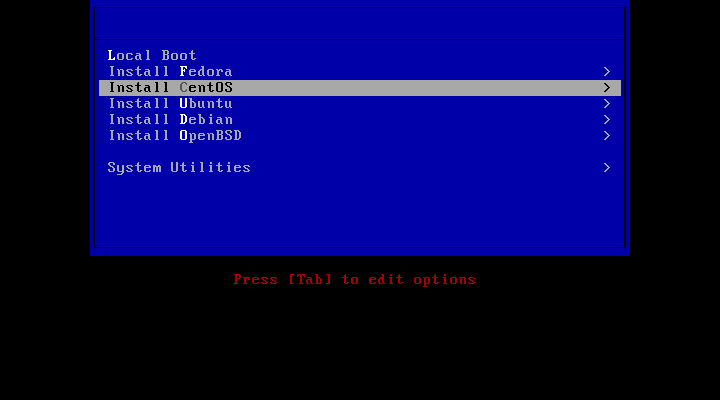
\includegraphics[width=\textwidth]{bootfoosh-bootmenu.png}
  \caption{boot.foo.sh boot menu showing selection of operating systems.}
  \label{fig:bootmenu}
\end{figure}

``Boot menu'' is used to display choices of operating systems to be
installed. Example of boot menu can be seen in figure~\ref{fig:bootmenu}.

``kernel and initrd'' are the files needed to launch Linux
installation. These two files are downloaded over the internet and
then kernel is executed and it continues the boot process.

``Kickstart'' is CentOS specific file for automating unattended
installation. It's set of instructions downloaded and executed by the
installation process.

``Installation files'' are the contents of operating system to be
installed. The files are downloaded and extracted to hard drive to
achieve the installation.

``Digital signatures'' are cryptographically calculated proofs to
verify signed content (for example contents of a file). If the content
is changed, the signature check fails and user can be alerted about
the incident.

\section{Analysis}

In all three systems the same protocols are used for zero
configuration (DHCP) and name resolution (DNS). DHCP and DNS are de
facto standard protocols to achieve the task they solve so there's no
surprise here.

Boot menu is used to display choices of operating systems to be
installed. TFTP and HTTP are the protocols used in traditional and
over the internet systems. Both TFTP and HTTP protocols are
susceptible to Man in the Middle attack. Secudep uses HTTPS (HTTP over
TLS) with signed files.

\begin{figure}[h]
  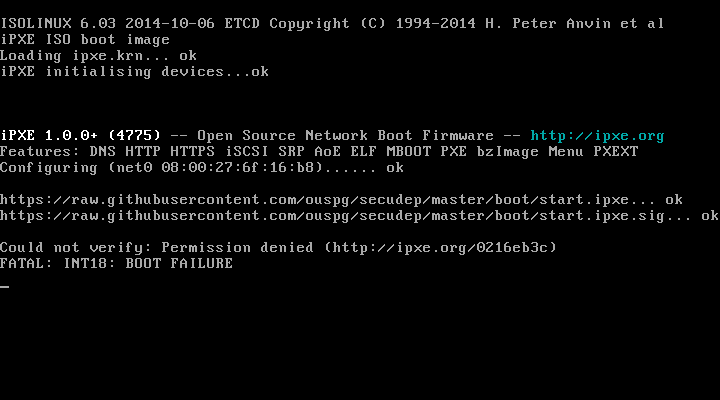
\includegraphics[width=\textwidth]{verify-fail.png}
  \caption{Installation process is halted when digital signature
    verification fails.}
  \label{fig:verify-fail}
\end{figure}

Only secudep uses digital signatures and the signature files are
fetched over HTTPS. This is the step missing from the traditional and
over the internet installation systems. Figure~\ref{fig:verify-fail}
shows how secudep's process is halted when digital signature
verification fails. This failure is clear indication that something is
definitely wrong.

Kernel and initrd are the files needed to launch Linux
installation. Here traditional system uses TFTP to serve these files,
but over internet and secudep systems use HTTP. Again TFTP and HTTP
are susceptible to Man in the Middle attacks. TFTP is the de facto
standard to deliver these files inside intranet systems. HTTP is used
because the files are fetched from CentOS's official mirror over the
internet. Secudep uses digital signatures to verify downloaded content.

After kernel and initrd are downloaded and digital signatures are
verified the execution is handled to kernel. This means that secudep
can't provide digital signatures to any following files. However, there's
still two important steps in installation process: kickstart file and
installation files.

Kickstart is CentOS specific file for automating unattended
installation. The kickstart file is downloaded by the initrd system so
secudep can't do digital signature verification. However, secudep uses
HTTPS where traditional relies on NFS and over internet system uses
HTTP. Both NFS and HTTP are suspecting to Man in the Middle attacks.

Installation files are downloaded and then installed into hard drive
to achieve the operating system installation. Operating system
installer is usually trusted to verify digital signatures (e.g. CentOS
uses GPG signatures) the downloaded content before extracting the
files into hard drive. CentOS documentation~\cite{centos-gpg} states
that

\begin{quote}
Each stable RPM package that is published by CentOS Project is signed
with a GPG signature. By default, yum and the graphical update tools
will verify these signatures and refuse to install any packages that
are not signed, or have an incorrect signature. You should always
verify the signature of a package prior to installation. These
signatures ensure that the packages you install are what was produced
by the CentOS Project and have not been altered by any mirror or
website providing the packages.
\end{quote}

However, when initrd file is downloaded over insecure protocol or file
content is not verified against signature it's possible for malicious
third party to inject it's own GPG keys into initrd and point
installation system to malicious host serving the operating system
installation files and thus gain full control of the installed system.
